\documentclass[../../main.tex]{subfiles}
\begin{document}

\section{Medici\'on corriente de bias y tensi\'on de offset}

\subsection{Modelo de amplificador operacional con corrientes de bias y tensi\'on de offset}


\begin{figure}[htb]	%modelo opamp vio ibias
	\centering
	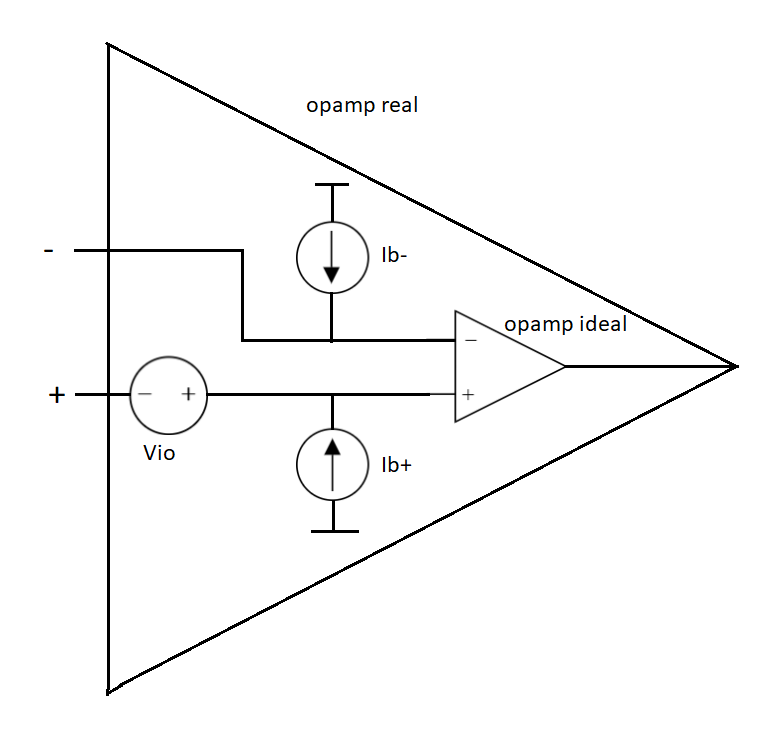
\includegraphics[width=0.4\textwidth]{imagenes/modelo_opamp_vio_ibias.png}
	\caption{Modelo de amplificador operacional con corrientes de bias y tensi\'on de offset}
	\label{fig:ej5_modelo_opamp_vio_ibias}
\end{figure}


\todo[inline]{Que es corriente de bias y tension de offset. fijarme que puso roch en la intro}

\subsection{Importancia de las corrientes de bias y la tensi\'on de offset}



Las corrientes de bias($I_B^+$ y $I_B^-$) y la tensi\'on de offset ($V_{IO}$) pueden generar efectos que no concuerdan con el modelo ideal de un amplificador operacional. Se presentan a continuaci\'on dos ejemplos:

\subsubsection*{Efecto de $V_{IO}$}

\begin{figure}[htb]	%vio no despreciable
	\centering
	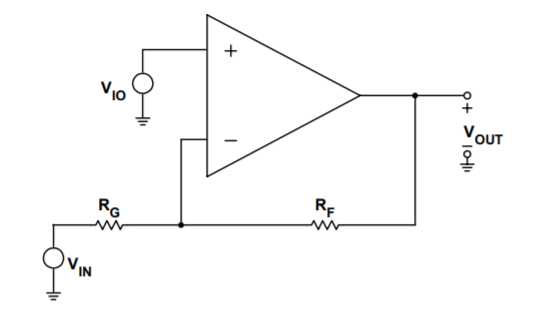
\includegraphics[height=0.2\textheight]{imagenes/vio_amplificacion.png}
	\caption{Modelo de amplificador con configuraci\'on inversora con $V_{IO}$ no despreciable}
	\label{fig:ej_3_efecto_vio}
\end{figure}

El circuito de la figura \ref{fig:ej_3_efecto_vio} representa un amplificador operacional en configuraci\'on inversora con tensi\'on de offset no despreciable modelado por un \textit{op-amp} ideal y una fuente de tensi\'on continua $V_{IO}$. De ignorarse la tensi\'on de offset, puede obtenerse la funci\'on transferencia:

\[\frac{V_{OUT}}{V_{IN}}=\frac{-R_F}{R_G}\]

Sin embargo, si se considera la tensi\'on de offset, no es posible obtener obtener la funci\'on transferencia ya que el sistema no es lineal:

\[V_{OUT}=V_{IN}\frac{-R_F}{R_G} + V_{IO}\left(1+\frac{R_F}{R_G}\right)\]
\[\text{Si }V_{IN} = 0,V_{OUT} = V_{IO}\left(1+\frac{R_F}{R_G}\right) \neq 0 \]
\[\Rightarrow \text{El sistema no es lineal}\]

Dependiendo el orden de $V_{IN}$ y de $V_{IO}$ y de la precisi\'on necesaria, el efecto de $V_{IO}$ en $V_{OUT}$ no puede ser despreciado.

\subsubsection*{Efecto de $I_B^+$ y $I_B^-$}
El amplificador operacional no puede funcionar si se impide el paso de las corrientes de bias. \todo{"impide el paso" suena medio choto pero no s\'e como decirlo m\'as mejor}Si se decide poner un capacitor en serie con una de las entradas, $I_B$ no podr\'a circular, haciendo que el amplificador no funcione correctamente. Ver ejemplo en figura \ref{fig:ej_3_GIC}. \todo{redaccion}

\begin{figure}[htb] %GIC
	\centering
	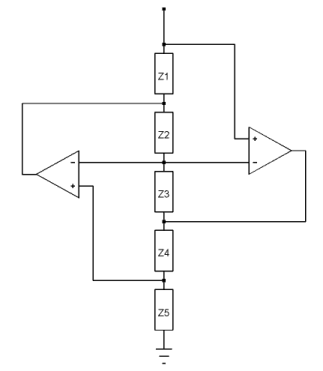
\includegraphics[width=0.35\textwidth]{imagenes/gic.png}
	\caption[Capacitores en un GIC]{Circuito GIC. Si $Z_2$ y $Z_3$ fueran capacitores, no podri\'ian circular las corrientes de bias. Una posible soluci\'on consiste en poner una resistencia en paralelo que permita la circulaci\'on y que sea lo suficientemente grande como para que la impedancia resultante sea aproximadamente capacituva pura.}
	\label{fig:ej_3_GIC}
\end{figure}


Por otro lado, si hay una resistencia $R$ en serie con la entrada del operacional, habr\'a una ca\'ida de tensi\'on $V=I_B^\pm\cdot R$ que puede o no ser despreciable dependiendo de la relaci\'on entre $I_B^\pm$ y $R$ y las caracter\'isticas del circuito. Este efecto es usado en el circuito de medici\'on explicado en la siguiente secci\'on para medir $I_B^+$ y $I_B^-$

\subsection{Funcionamiento del circuito}
La funci\'on del circuito es medir la tensi\'on de offset y las corrientes de bias. La corriente de bias se obtiene midiendo la ca\'ida de tensi\'on que genera sobre una resistencia de $1M\Omega$. En la tabla 


\begin{table}[htb]
	\centering
	\begin{tabular}{cccc}
	         & $V_{IO}(mV)$ & $I_B (pA) $ & $I_B\cdot 1M\Omega (mV)$    \\
\hline
	T\'ipico &     3        &      30     &  0.03       \\
	M\'aximo &	  10        &     200   &  0.2		
	\end{tabular}
	\caption{Valores de $V_{IO}$, $I_B$, y ca\'ida de tensi\'on generada por $I_B$ para el LF356 y TL081. Valores t\'ipicos con $V_{cc\pm}=15V$ y a $25^{\circ}C$ especificados por el fabricante en la hoja de datos.}
	\label{tab:ej_3_datasheet}
\end{table}

Todas las tensiones a determinar son amplificadas para as\'i aumentar la precisi\'on en la medici\'on. Una posibilidad ser\'ia amplificar a lazo abierto. Este m\'etodo cuenta con dos desventajas:
\begin{itemize}
	\item La ganancia a lazo abierto $A_{vol}$ t\'ipica es 200V/mV. Con los valores de la tabla \ref{tab:ej_3_datasheet} el amplificador saturar\'ia.
	\item Incluso si no hubiera saturaci\'on, \todo{redaccion: avol es super impreciso/ cambia una bocha entonces el resultado seria muy impreciso}
\end{itemize}
Por estos motivos se utiliza amplificaci\'on a lazo cerrado. En la figura \ref{fig:ej_3_medicion_vio_simple} se muestra un circuito de medici\'on de $V_{IO}$. Sabiendo que la ganancia de un circuito de amplificacion no inversor es $(1+\frac{R_2}{R_1}$, se obtiene $V_{IO} = \frac{R_1}{R_1+R_2}\cdot V_{OUT}$. 


\begin{figure}[htb]	%medicion vio simplificado
	\centering
	\begin{subfigure}[t]{0.43\textwidth}
		\centering
		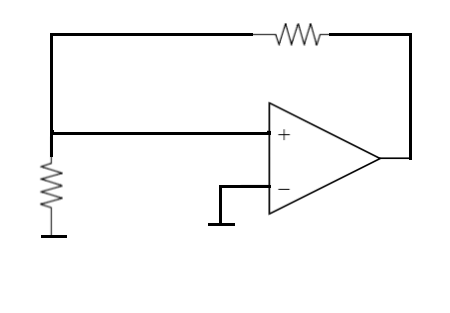
\includegraphics[width=\textwidth]{imagenes/medicion_vio_configuracion_simplificada.png}
		\caption{Con \textit{op-amp} real}
	\end{subfigure}%
	\hfill%%
	\begin{subfigure}[t]{0.43\textwidth}
		\centering
		\missingfigure[figwidth=\textwidth]{opamp ideal con fuente afuera}
		\caption{Con \textit{op-amp} ideal y fuente de tensi\'on modelando el \textit{op-amp} real}
	\end{subfigure}	
	\caption[Circuito de medici\'on de $V_{IO}$ simplificado.]{Circuito de medici\'on de $V_{IO}$ simplificado.  $V_{OUT} = V_{IO} \cdot \left( 1+ \frac{R_2}{R_1} \right) $. No mide corrientes de bias y amplifica todas las frecuencias por igual.}
	\label{fig:ej_3_medicion_vio_simple}
\end{figure}


Ya que las se\~nales que se quieren medir tienen una amplitud comparable con el ruido que pueda llegar a inducirse en el circuito, es conveniente reducir la amplificaci\'on para las frecuencias mayores a cero. \todo{redaccion} Esto se logra en el circuito presentado en la consigna (figura \ref{fig:ej_3_medicion_vio_consigna}

\begin{figure}[htb] %medicion vio ib+ ib- posta
	\centering
	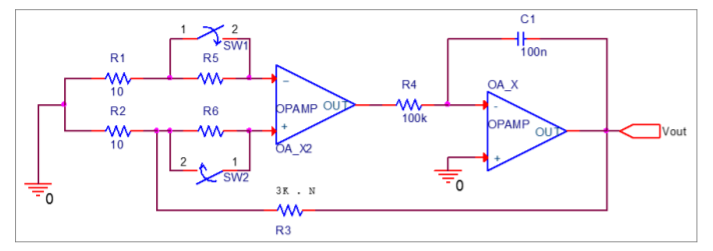
\includegraphics[scale=1]{imagenes/medicion_bias_configuracion_consigna.png}
	\caption{Circuito de medici\'on de $V_{IO}$, $I_B^+$ y $I_B^-$. La amplificaci\'on disminuye con el aumento de la frecuencia.}
	\label{fig:ej_3_medicion_vio_consigna}
\end{figure}


con los interruptores cerrados llego a que Vio=

\subsubsection{Funcionamiento en DC}

Consideraciones a la hora de hacer el diagrama de flujo de se\~nal:
\begin{itemize}
	\item $\Delta V_{R1} = I_B^-\cdot R_1 \approx 0$
	\item $V_{OUT\, DUT} = A_{vol} \left( V_{d\, DUT} + I_B^+\right)
\end{itemize}
En r\'egimen permanente, la ganancia en el \textit{OA\_X} es $A_{vol}$, ya que el capacitor se abre: 

\begin{figure}[htb]
	\centering
	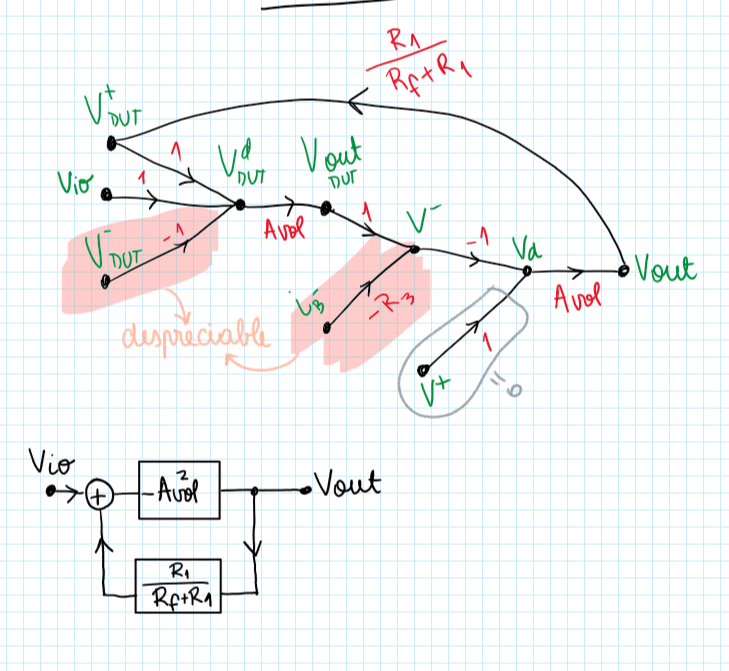
\includegraphics[scale=1]{imagenes/dc_signal_feedback.png}
	\caption{An\'alisis en DC por diagrama de flujo de se\~nal}
	\label{fig:ej_3_diagrama_flujo_senial}
\end{figure}

Se desprecian las caidas de tension generadas por las corrientes de bias en las resistencias R1, R2 y R4, por lo que en en R1 y en R4 delta V es 0, en R2 delta V es (divisor de tension con Vout)

\subsubsection{Funcionamiento en AC}



\begin{itemize}
	\item estabilidad
	\item inversion de los opamps
\end{itemize}

\end{document}
